% Anonymous submission: pdflatex main
% arXiv preprint with author names: pdflatex -jobname=main-preprint "\def\PREPRINT{}% Anonymous submission: pdflatex main
% arXiv preprint with author names: pdflatex -jobname=main-preprint "\def\PREPRINT{}% Anonymous submission: pdflatex main
% arXiv preprint with author names: pdflatex -jobname=main-preprint "\def\PREPRINT{}% Anonymous submission: pdflatex main
% arXiv preprint with author names: pdflatex -jobname=main-preprint "\def\PREPRINT{}\input{main}"
% (see Makefile)
\documentclass{article}
\usepackage{xcolor}

\ifdefined\PREPRINT
  \usepackage[preprint]{corl_2026}
\else
  \usepackage{corl_2026}
  % The style's footer names the main conference; this is a workshop submission.
  \makeatletter
  \renewcommand{\@noticestring}{Submitted to the CoRL 2026 Workshop on Efficient Foundation
    Models for Real-Time Embodied AI. Do not distribute.}
  \makeatother
\fi

\usepackage{booktabs}
\usepackage{graphicx}
\graphicspath{{../}}
\usepackage{amsmath}
\usepackage{xspace}

\newcommand{\todo}[1]{\textcolor{red}{[TODO: #1]}}
\newcommand{\pizero}{$\pi_0$\xspace}
\newcommand{\pizerofive}{$\pi_{0.5}$\xspace}

\title{Higher Success, New Failures:\\Measuring Per-State Regressions in VLA Policy Updates}

\author{
  Qiang Guo\\
  Independent Researcher\\
  \texttt{glay.guo@foxmail.com}
}

\begin{document}
\maketitle

\begin{abstract}
Quantized, distilled or otherwise accelerated vision-language-action (VLA) policies are judged by
the change in their aggregate success rate. A deployment also needs to know whether the new policy
fails where the old one succeeded. Comparing the two policies with one rollout per initial state,
the usual protocol, cannot tell: in VLAQuantBench's public LIBERO records, rerunning an unchanged
configuration with a new seed changes the outcome of up to a quarter of the initial states. We
define a state as a LIBERO initial state together with its scene seed, roll out every state several
times per policy with common random numbers, and test each state for regression under
false-discovery control. On X-VLA in LIBERO-10, this old-versus-old floor falls to 2--3 flips per
100 states; 4-bit weights leave every state intact, while 3-bit weights break seven states
outright and concentrate a 20-point drop on a few tasks. \todo{update with the step and BF16
variants.}
\end{abstract}

\keywords{Vision-language-action models, quantization, evaluation, regression testing}

%===============================================================================

\section{Introduction}

Deployed VLA policies are updated often: weights are quantized, flow-matching policies are run
with fewer denoising steps, longer action chunks are executed open-loop, and checkpoints are
fine-tuned again. Each update is reported as a change in success rate over a benchmark
suite~\citep{xu2026vlaquantbench}. An operator who has validated the old policy on a set of
situations asks a different question: in which of them does the new policy now fail? The
question is familiar from backward compatibility of model updates in classification
\citep{bansal2019updates,srivastava2020compat,yan2021pcr}, where a more accurate model can still
err on inputs the old one got right. For closed-loop control it has not been measured with any
statistical care.

Recent work compares VLA policies initial state by initial state on
LIBERO~\citep{liu2023libero}: \citet{sawada2026paired} pair states across perturbations and find
that up to 34.5\% of them change outcome, and \citet{yardimci2026collapse} report per-task
collapse under online RL fine-tuning while the aggregate looks healthy. These comparisons use one
rollout per state. A VLA rollout is random, through the policy's sampling and the simulator's
scene randomization, so part of any per-state difference is noise. How large that part is has not
been reported.

We make three contributions.
\begin{itemize}
  \item \textbf{The noise floor of single-rollout comparisons.} From VLAQuantBench's public
    records of four VLAs on four LIBERO suites, rerunning an unchanged configuration with a new
    seed flips the outcome of 1--25\% of states, depending on the success rate
    (Section~\ref{sec:floor}). Many reported per-state changes are within this floor.
  \item \textbf{A protocol} that makes per-state comparisons testable: states that fix the scene
    seed, repeated rollouts with common random numbers, per-state exact tests with
    Benjamini-Hochberg control, and an explicit old-versus-old baseline
    (Section~\ref{sec:method}). The harness is built on LeRobot~\citep{cadene2024lerobot}.
  \item \textbf{Per-state regressions of X-VLA}~\citep{zheng2025xvla} under weight
    quantization on LIBERO-10 (Section~\ref{sec:xvla}): at precisely defined states a rerun is
    close to a replay, W4 changes no state significantly, and W3's losses sit in seven states
    that go from always to never succeeding.
\end{itemize}

\section{Method}
\label{sec:method}

\paragraph{States.} LIBERO ships a fixed file of initial states per task that sets the robot and
the movable objects. Fixtures such as cabinets and stoves, however, are placed at random each time
the scene is rebuilt: three hard resets of LIBERO-10 task 0, state 0 gave three cabinet positions.
We therefore define a state $s$ as (task, initial state, scene seed) and reset each state with
its own fixed seed.

\paragraph{Rollouts.} Each state is rolled out $n$ times per policy variant. The policy's noise
seeds are a function of the evaluation plan only (task, batch, base seed), never of the variant,
so two variants see the same random numbers (common random numbers), and a rerun of the same
plan reproduces every episode exactly.

\paragraph{Tests.} Let $k_s^{\text{old}}, k_s^{\text{new}}$ be the successes out of $n$. For each
state we compute the one-sided Fisher exact $p$-value for ``the new variant succeeds less often''
and apply the Benjamini-Hochberg procedure~\citep{benjamini1995fdr} at FDR $q=0.1$ across states.
We also report the posterior probability that $p_s^{\text{new}} < p_s^{\text{old}}$ under
uniform Beta priors, and the aggregate change with a bootstrap over states. The \emph{naive}
count uses repeat 0 only: states that succeed under the old variant and fail under the new one, as
a single-rollout protocol would report.

\paragraph{Noise floor.} The old policy is compared with itself: the same states and scene seeds,
new policy seeds. Any flip or regression found here is a false alarm by construction.

\section{How noisy is one rollout per state?}
\label{sec:floor}

VLAQuantBench~\citep{xu2026vlaquantbench} released every episode of its 409 closed-loop runs
(MIT licence). On LIBERO it runs each configuration once on 200 states (20 initial states for
each of 10 tasks; 190 for X-VLA), and 20 configurations again with seeds 1 and 2. We use commit
\texttt{4a2cb7c}.

\paragraph{Unchanged configurations flip many states.} Table~\ref{tab:floor} and
Figure~\ref{fig:floor} show the states whose outcome differs between two seeds of the same
configuration. Near the ceiling the count is small (1--8 of 200 at 97.5--99.5\% success), but it
grows quickly as success falls: 21--32 states at 72--88\%, and 32--50 at 60--71\%.

\paragraph{Seeds do not pair configurations.} Two different configurations run with the same seed
disagree on as many states as with different seeds (e.g.\ \pizerofive base against its W4A4
action-head variant on LIBERO-Object: 77.3 at the same seed, 78.0 across seeds), so seed-to-seed
flips are the right floor for VLAQuantBench's cross-configuration comparisons.

\paragraph{States do differ.} The flips are not only noise around a common rate. For \pizerofive
with a W4A4 action head on LIBERO-Object (61\% success), 43 states fail in all three seeds and 85
succeed in all three; if all states had the same success rate we would expect 12 and 46. Real
per-state effects exist; a single rollout cannot separate them from chance.

\paragraph{Consequence.} Take \pizero~\citep{black2024pi0} on LIBERO-10 with W8 weights: aggregate
success moves from 48.5\% to 47.5\%, while 24 states flip to failure and 22 to success. At that
success rate, a new seed alone flips a comparable number of states (Table~\ref{tab:floor}). A
per-state reading of such a comparison needs repeated rollouts.

\begin{table}[t]
  \centering
  \small
  \caption{States that change outcome between seeds of the same configuration (VLAQuantBench,
  LIBERO, 200 states). Rows span the range of success rates; all 20 repeated configurations are
  in the supplementary material.}
  \label{tab:floor}
  \setlength{\tabcolsep}{4pt}
  \begin{tabular}{llccc}
    \toprule
    Suite / model & Configuration & Success by seed & Flips per seed pair & Never / always / mixed \\
    \midrule
    Object / \pizerofive & baseline & .990 .985 .995 & 5, 1, 4 & 0 / 195 / 5 \\
    Object / \pizerofive & W4A4, action head & .600 .630 .610 & 44, 50, 50 & 43 / 85 / 72 \\
    Spatial / \pizerofive & W4A4, action head & .705 .705 .685 & 44, 36, 32 & 34 / 110 / 56 \\
    Spatial / \pizerofive & W4A4, MLP only & .880 .875 & 29 & 10 / 161 / 29 \\
    10 / OpenVLA-OFT & W3, no fc2 in head & .935 .915 .910 & 8, 7, 9 & 11 / 177 / 12 \\
    \bottomrule
  \end{tabular}
\end{table}

\begin{figure}[t]
  \centering
  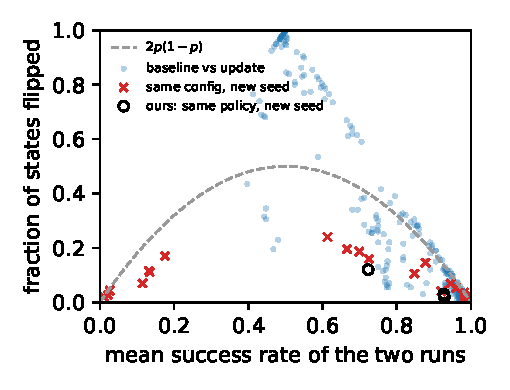
\includegraphics[width=0.55\linewidth]{fig_noise_floor.pdf}
  \caption{Fraction of states that change outcome between two runs, against their mean success
  rate. Crosses: the same configuration with a new seed. Dots: baseline against every other
  configuration in VLAQuantBench. The dashed curve is $2p(1-p)$, the flip rate if every state had
  success rate $p$; repeats fall below it because states differ in difficulty.}
  \label{fig:floor}
\end{figure}

\section{Per-state regressions of X-VLA under quantization}
\label{sec:xvla}

\paragraph{Setup.} We evaluate \texttt{lerobot/xvla-libero} in LeRobot 0.6.1 on LIBERO-10:
10 tasks $\times$ 10 initial states $\times$ 5 rollouts, absolute end-effector control, 10
flow-matching steps, and LeRobot's 520-step limit. Every failure in the FP32 run is a timeout at
this limit; VLAQuantBench allows 900 steps and reports 97.9\% for the same model, against 92.4\%
here. The quantized variants round all 267 linear layers (792M parameters) to a symmetric
integer grid and store them dequantized: INT8 with one scale per output channel, INT4 with one
scale per group of 128 inputs.

\begin{table}[t]
  \centering
  \small
  \caption{X-VLA on LIBERO-10, FP32 against each variant: 100 states, 5 rollouts each. Naive
  flips use the first rollout only (to failure / to success). BH: states with a significant
  per-state change at FDR 0.1 (regressed / improved). The first two rows compare FP32 with
  itself.}
  \label{tab:xvla}
  \begin{tabular}{lccccc}
    \toprule
    Variant & Success & $\Delta$ [95\% CI] & Naive flips & BH & $P(\text{worse})>0.9$ \\
    \midrule
    FP32, new policy seeds & .928 & $+0.2$ [$-1.0$, $+1.4$] & 0 / 3 & 0 / 0 & 0 \\
    FP32, new scene seeds & .930 & $+0.4$ [$-0.4$, $+1.2$] & 0 / 2 & 0 / 0 & 0 \\
    W4, group 128 & .918 & $-0.8$ [$-3.2$, $+1.2$] & 4 / 2 & 0 / 0 & 1 \\
    W3, group 128 & .726 & $-20.0$ [$-26.8$, $-13.4$] & 23 / 2 & 7 / 0 & 26 \\
    \todo{2 denoising steps} & & & & & \\
    \todo{BF16} & & & & & \\
    \bottomrule
  \end{tabular}
\end{table}

\paragraph{The floor is low at fixed states.} With states that fix the scene seed, FP32 against
itself changes the outcome of 13 of 500 rollouts under new policy seeds and 8 of 500 under new
scene seeds; no state's success count moves by more than two, and neither run has a significant
state. 88 of the 100 states succeed in all five FP32 rollouts and 5 fail in all five. The large
seed-to-seed flip counts of Section~\ref{sec:floor} are therefore not intrinsic to the policy:
once a state is defined precisely, a rerun is close to a replay.

\paragraph{W4 is safe per state as well as on average.} Its six naive flips are twice the floor,
but none survives the test; the most affected state drops from 5/5 to 1/5 ($p=0.024$, not
significant after correction).

\paragraph{W3 fails in specific places.} The 20-point drop is concentrated: tasks 5, 8 and 9 keep
96--100\% while tasks 0, 4 and 7 lose 40--52 points. Seven states go from 5/5 to 0/5 and are
flagged; 26 have posterior probability above 0.9 of having become worse. The single-rollout
protocol would report 23 new failures and 2 new successes, and cannot say which of them are real.

\section{Discussion}

A per-state claim about a policy update is a claim about $\sim$100--200 small binomial
experiments, and it should be reported the way such claims are: with repeated rollouts, a test,
multiplicity control, and the result of the old policy against itself. We recommend reporting
per-state regressions next to $\Delta$ success whenever an update is shipped, and the noise
floor next to any per-state flip count.

\paragraph{Limitations.} Simulation only; LIBERO offers few initial states per task; our
quantization is simulated weight-only rounding. Fixed designs with $n=5$ detect only large
per-state drops: a state at 95\% success that falls to 20\% is flagged with probability 0.64 by
a single-state test at level 0.05, one that falls to 50\% with probability 0.15 (0.94 with
$n=20$). Allocating rollouts sequentially to uncertain
states~\citep{snyder2025step} is the natural next step. Related paired tests on suite
level~\citep{islam2026onnx} and update-admission gates~\citep{ma2026admission} address the
aggregate or a synthetic setting; we target states of a real VLA benchmark.

\bibliography{references}

\end{document}
"
% (see Makefile)
\documentclass{article}
\usepackage{xcolor}

\ifdefined\PREPRINT
  \usepackage[preprint]{corl_2026}
\else
  \usepackage{corl_2026}
  % The style's footer names the main conference; this is a workshop submission.
  \makeatletter
  \renewcommand{\@noticestring}{Submitted to the CoRL 2026 Workshop on Efficient Foundation
    Models for Real-Time Embodied AI. Do not distribute.}
  \makeatother
\fi

\usepackage{booktabs}
\usepackage{graphicx}
\graphicspath{{../}}
\usepackage{amsmath}
\usepackage{xspace}

\newcommand{\todo}[1]{\textcolor{red}{[TODO: #1]}}
\newcommand{\pizero}{$\pi_0$\xspace}
\newcommand{\pizerofive}{$\pi_{0.5}$\xspace}

\title{Higher Success, New Failures:\\Measuring Per-State Regressions in VLA Policy Updates}

\author{
  Qiang Guo\\
  Independent Researcher\\
  \texttt{glay.guo@foxmail.com}
}

\begin{document}
\maketitle

\begin{abstract}
Quantized, distilled or otherwise accelerated vision-language-action (VLA) policies are judged by
the change in their aggregate success rate. A deployment also needs to know whether the new policy
fails where the old one succeeded. Comparing the two policies with one rollout per initial state,
the usual protocol, cannot tell: in VLAQuantBench's public LIBERO records, rerunning an unchanged
configuration with a new seed changes the outcome of up to a quarter of the initial states. We
define a state as a LIBERO initial state together with its scene seed, roll out every state several
times per policy with common random numbers, and test each state for regression under
false-discovery control. On X-VLA in LIBERO-10, this old-versus-old floor falls to 2--3 flips per
100 states; 4-bit weights leave every state intact, while 3-bit weights break seven states
outright and concentrate a 20-point drop on a few tasks. \todo{update with the step and BF16
variants.}
\end{abstract}

\keywords{Vision-language-action models, quantization, evaluation, regression testing}

%===============================================================================

\section{Introduction}

Deployed VLA policies are updated often: weights are quantized, flow-matching policies are run
with fewer denoising steps, longer action chunks are executed open-loop, and checkpoints are
fine-tuned again. Each update is reported as a change in success rate over a benchmark
suite~\citep{xu2026vlaquantbench}. An operator who has validated the old policy on a set of
situations asks a different question: in which of them does the new policy now fail? The
question is familiar from backward compatibility of model updates in classification
\citep{bansal2019updates,srivastava2020compat,yan2021pcr}, where a more accurate model can still
err on inputs the old one got right. For closed-loop control it has not been measured with any
statistical care.

Recent work compares VLA policies initial state by initial state on
LIBERO~\citep{liu2023libero}: \citet{sawada2026paired} pair states across perturbations and find
that up to 34.5\% of them change outcome, and \citet{yardimci2026collapse} report per-task
collapse under online RL fine-tuning while the aggregate looks healthy. These comparisons use one
rollout per state. A VLA rollout is random, through the policy's sampling and the simulator's
scene randomization, so part of any per-state difference is noise. How large that part is has not
been reported.

We make three contributions.
\begin{itemize}
  \item \textbf{The noise floor of single-rollout comparisons.} From VLAQuantBench's public
    records of four VLAs on four LIBERO suites, rerunning an unchanged configuration with a new
    seed flips the outcome of 1--25\% of states, depending on the success rate
    (Section~\ref{sec:floor}). Many reported per-state changes are within this floor.
  \item \textbf{A protocol} that makes per-state comparisons testable: states that fix the scene
    seed, repeated rollouts with common random numbers, per-state exact tests with
    Benjamini-Hochberg control, and an explicit old-versus-old baseline
    (Section~\ref{sec:method}). The harness is built on LeRobot~\citep{cadene2024lerobot}.
  \item \textbf{Per-state regressions of X-VLA}~\citep{zheng2025xvla} under weight
    quantization on LIBERO-10 (Section~\ref{sec:xvla}): at precisely defined states a rerun is
    close to a replay, W4 changes no state significantly, and W3's losses sit in seven states
    that go from always to never succeeding.
\end{itemize}

\section{Method}
\label{sec:method}

\paragraph{States.} LIBERO ships a fixed file of initial states per task that sets the robot and
the movable objects. Fixtures such as cabinets and stoves, however, are placed at random each time
the scene is rebuilt: three hard resets of LIBERO-10 task 0, state 0 gave three cabinet positions.
We therefore define a state $s$ as (task, initial state, scene seed) and reset each state with
its own fixed seed.

\paragraph{Rollouts.} Each state is rolled out $n$ times per policy variant. The policy's noise
seeds are a function of the evaluation plan only (task, batch, base seed), never of the variant,
so two variants see the same random numbers (common random numbers), and a rerun of the same
plan reproduces every episode exactly.

\paragraph{Tests.} Let $k_s^{\text{old}}, k_s^{\text{new}}$ be the successes out of $n$. For each
state we compute the one-sided Fisher exact $p$-value for ``the new variant succeeds less often''
and apply the Benjamini-Hochberg procedure~\citep{benjamini1995fdr} at FDR $q=0.1$ across states.
We also report the posterior probability that $p_s^{\text{new}} < p_s^{\text{old}}$ under
uniform Beta priors, and the aggregate change with a bootstrap over states. The \emph{naive}
count uses repeat 0 only: states that succeed under the old variant and fail under the new one, as
a single-rollout protocol would report.

\paragraph{Noise floor.} The old policy is compared with itself: the same states and scene seeds,
new policy seeds. Any flip or regression found here is a false alarm by construction.

\section{How noisy is one rollout per state?}
\label{sec:floor}

VLAQuantBench~\citep{xu2026vlaquantbench} released every episode of its 409 closed-loop runs
(MIT licence). On LIBERO it runs each configuration once on 200 states (20 initial states for
each of 10 tasks; 190 for X-VLA), and 20 configurations again with seeds 1 and 2. We use commit
\texttt{4a2cb7c}.

\paragraph{Unchanged configurations flip many states.} Table~\ref{tab:floor} and
Figure~\ref{fig:floor} show the states whose outcome differs between two seeds of the same
configuration. Near the ceiling the count is small (1--8 of 200 at 97.5--99.5\% success), but it
grows quickly as success falls: 21--32 states at 72--88\%, and 32--50 at 60--71\%.

\paragraph{Seeds do not pair configurations.} Two different configurations run with the same seed
disagree on as many states as with different seeds (e.g.\ \pizerofive base against its W4A4
action-head variant on LIBERO-Object: 77.3 at the same seed, 78.0 across seeds), so seed-to-seed
flips are the right floor for VLAQuantBench's cross-configuration comparisons.

\paragraph{States do differ.} The flips are not only noise around a common rate. For \pizerofive
with a W4A4 action head on LIBERO-Object (61\% success), 43 states fail in all three seeds and 85
succeed in all three; if all states had the same success rate we would expect 12 and 46. Real
per-state effects exist; a single rollout cannot separate them from chance.

\paragraph{Consequence.} Take \pizero~\citep{black2024pi0} on LIBERO-10 with W8 weights: aggregate
success moves from 48.5\% to 47.5\%, while 24 states flip to failure and 22 to success. At that
success rate, a new seed alone flips a comparable number of states (Table~\ref{tab:floor}). A
per-state reading of such a comparison needs repeated rollouts.

\begin{table}[t]
  \centering
  \small
  \caption{States that change outcome between seeds of the same configuration (VLAQuantBench,
  LIBERO, 200 states). Rows span the range of success rates; all 20 repeated configurations are
  in the supplementary material.}
  \label{tab:floor}
  \setlength{\tabcolsep}{4pt}
  \begin{tabular}{llccc}
    \toprule
    Suite / model & Configuration & Success by seed & Flips per seed pair & Never / always / mixed \\
    \midrule
    Object / \pizerofive & baseline & .990 .985 .995 & 5, 1, 4 & 0 / 195 / 5 \\
    Object / \pizerofive & W4A4, action head & .600 .630 .610 & 44, 50, 50 & 43 / 85 / 72 \\
    Spatial / \pizerofive & W4A4, action head & .705 .705 .685 & 44, 36, 32 & 34 / 110 / 56 \\
    Spatial / \pizerofive & W4A4, MLP only & .880 .875 & 29 & 10 / 161 / 29 \\
    10 / OpenVLA-OFT & W3, no fc2 in head & .935 .915 .910 & 8, 7, 9 & 11 / 177 / 12 \\
    \bottomrule
  \end{tabular}
\end{table}

\begin{figure}[t]
  \centering
  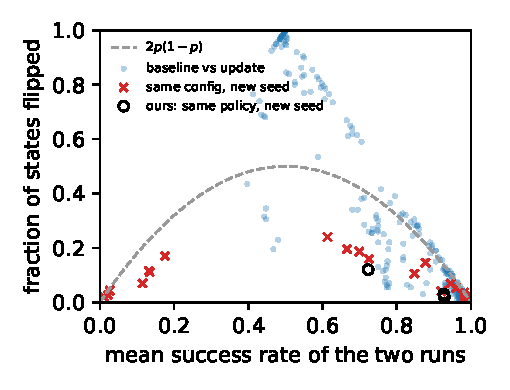
\includegraphics[width=0.55\linewidth]{fig_noise_floor.pdf}
  \caption{Fraction of states that change outcome between two runs, against their mean success
  rate. Crosses: the same configuration with a new seed. Dots: baseline against every other
  configuration in VLAQuantBench. The dashed curve is $2p(1-p)$, the flip rate if every state had
  success rate $p$; repeats fall below it because states differ in difficulty.}
  \label{fig:floor}
\end{figure}

\section{Per-state regressions of X-VLA under quantization}
\label{sec:xvla}

\paragraph{Setup.} We evaluate \texttt{lerobot/xvla-libero} in LeRobot 0.6.1 on LIBERO-10:
10 tasks $\times$ 10 initial states $\times$ 5 rollouts, absolute end-effector control, 10
flow-matching steps, and LeRobot's 520-step limit. Every failure in the FP32 run is a timeout at
this limit; VLAQuantBench allows 900 steps and reports 97.9\% for the same model, against 92.4\%
here. The quantized variants round all 267 linear layers (792M parameters) to a symmetric
integer grid and store them dequantized: INT8 with one scale per output channel, INT4 with one
scale per group of 128 inputs.

\begin{table}[t]
  \centering
  \small
  \caption{X-VLA on LIBERO-10, FP32 against each variant: 100 states, 5 rollouts each. Naive
  flips use the first rollout only (to failure / to success). BH: states with a significant
  per-state change at FDR 0.1 (regressed / improved). The first two rows compare FP32 with
  itself.}
  \label{tab:xvla}
  \begin{tabular}{lccccc}
    \toprule
    Variant & Success & $\Delta$ [95\% CI] & Naive flips & BH & $P(\text{worse})>0.9$ \\
    \midrule
    FP32, new policy seeds & .928 & $+0.2$ [$-1.0$, $+1.4$] & 0 / 3 & 0 / 0 & 0 \\
    FP32, new scene seeds & .930 & $+0.4$ [$-0.4$, $+1.2$] & 0 / 2 & 0 / 0 & 0 \\
    W4, group 128 & .918 & $-0.8$ [$-3.2$, $+1.2$] & 4 / 2 & 0 / 0 & 1 \\
    W3, group 128 & .726 & $-20.0$ [$-26.8$, $-13.4$] & 23 / 2 & 7 / 0 & 26 \\
    \todo{2 denoising steps} & & & & & \\
    \todo{BF16} & & & & & \\
    \bottomrule
  \end{tabular}
\end{table}

\paragraph{The floor is low at fixed states.} With states that fix the scene seed, FP32 against
itself changes the outcome of 13 of 500 rollouts under new policy seeds and 8 of 500 under new
scene seeds; no state's success count moves by more than two, and neither run has a significant
state. 88 of the 100 states succeed in all five FP32 rollouts and 5 fail in all five. The large
seed-to-seed flip counts of Section~\ref{sec:floor} are therefore not intrinsic to the policy:
once a state is defined precisely, a rerun is close to a replay.

\paragraph{W4 is safe per state as well as on average.} Its six naive flips are twice the floor,
but none survives the test; the most affected state drops from 5/5 to 1/5 ($p=0.024$, not
significant after correction).

\paragraph{W3 fails in specific places.} The 20-point drop is concentrated: tasks 5, 8 and 9 keep
96--100\% while tasks 0, 4 and 7 lose 40--52 points. Seven states go from 5/5 to 0/5 and are
flagged; 26 have posterior probability above 0.9 of having become worse. The single-rollout
protocol would report 23 new failures and 2 new successes, and cannot say which of them are real.

\section{Discussion}

A per-state claim about a policy update is a claim about $\sim$100--200 small binomial
experiments, and it should be reported the way such claims are: with repeated rollouts, a test,
multiplicity control, and the result of the old policy against itself. We recommend reporting
per-state regressions next to $\Delta$ success whenever an update is shipped, and the noise
floor next to any per-state flip count.

\paragraph{Limitations.} Simulation only; LIBERO offers few initial states per task; our
quantization is simulated weight-only rounding. Fixed designs with $n=5$ detect only large
per-state drops: a state at 95\% success that falls to 20\% is flagged with probability 0.64 by
a single-state test at level 0.05, one that falls to 50\% with probability 0.15 (0.94 with
$n=20$). Allocating rollouts sequentially to uncertain
states~\citep{snyder2025step} is the natural next step. Related paired tests on suite
level~\citep{islam2026onnx} and update-admission gates~\citep{ma2026admission} address the
aggregate or a synthetic setting; we target states of a real VLA benchmark.

\bibliography{references}

\end{document}
"
% (see Makefile)
\documentclass{article}
\usepackage{xcolor}

\ifdefined\PREPRINT
  \usepackage[preprint]{corl_2026}
\else
  \usepackage{corl_2026}
  % The style's footer names the main conference; this is a workshop submission.
  \makeatletter
  \renewcommand{\@noticestring}{Submitted to the CoRL 2026 Workshop on Efficient Foundation
    Models for Real-Time Embodied AI. Do not distribute.}
  \makeatother
\fi

\usepackage{booktabs}
\usepackage{graphicx}
\graphicspath{{../}}
\usepackage{amsmath}
\usepackage{xspace}

\newcommand{\todo}[1]{\textcolor{red}{[TODO: #1]}}
\newcommand{\pizero}{$\pi_0$\xspace}
\newcommand{\pizerofive}{$\pi_{0.5}$\xspace}

\title{Higher Success, New Failures:\\Measuring Per-State Regressions in VLA Policy Updates}

\author{
  Qiang Guo\\
  Independent Researcher\\
  \texttt{glay.guo@foxmail.com}
}

\begin{document}
\maketitle

\begin{abstract}
Quantized, distilled or otherwise accelerated vision-language-action (VLA) policies are judged by
the change in their aggregate success rate. A deployment also needs to know whether the new policy
fails where the old one succeeded. Comparing the two policies with one rollout per initial state,
the usual protocol, cannot tell: in VLAQuantBench's public LIBERO records, rerunning an unchanged
configuration with a new seed changes the outcome of up to a quarter of the initial states. We
define a state as a LIBERO initial state together with its scene seed, roll out every state several
times per policy with common random numbers, and test each state for regression under
false-discovery control. On X-VLA in LIBERO-10, this old-versus-old floor falls to 2--3 flips per
100 states; 4-bit weights leave every state intact, while 3-bit weights break seven states
outright and concentrate a 20-point drop on a few tasks. \todo{update with the step and BF16
variants.}
\end{abstract}

\keywords{Vision-language-action models, quantization, evaluation, regression testing}

%===============================================================================

\section{Introduction}

Deployed VLA policies are updated often: weights are quantized, flow-matching policies are run
with fewer denoising steps, longer action chunks are executed open-loop, and checkpoints are
fine-tuned again. Each update is reported as a change in success rate over a benchmark
suite~\citep{xu2026vlaquantbench}. An operator who has validated the old policy on a set of
situations asks a different question: in which of them does the new policy now fail? The
question is familiar from backward compatibility of model updates in classification
\citep{bansal2019updates,srivastava2020compat,yan2021pcr}, where a more accurate model can still
err on inputs the old one got right. For closed-loop control it has not been measured with any
statistical care.

Recent work compares VLA policies initial state by initial state on
LIBERO~\citep{liu2023libero}: \citet{sawada2026paired} pair states across perturbations and find
that up to 34.5\% of them change outcome, and \citet{yardimci2026collapse} report per-task
collapse under online RL fine-tuning while the aggregate looks healthy. These comparisons use one
rollout per state. A VLA rollout is random, through the policy's sampling and the simulator's
scene randomization, so part of any per-state difference is noise. How large that part is has not
been reported.

We make three contributions.
\begin{itemize}
  \item \textbf{The noise floor of single-rollout comparisons.} From VLAQuantBench's public
    records of four VLAs on four LIBERO suites, rerunning an unchanged configuration with a new
    seed flips the outcome of 1--25\% of states, depending on the success rate
    (Section~\ref{sec:floor}). Many reported per-state changes are within this floor.
  \item \textbf{A protocol} that makes per-state comparisons testable: states that fix the scene
    seed, repeated rollouts with common random numbers, per-state exact tests with
    Benjamini-Hochberg control, and an explicit old-versus-old baseline
    (Section~\ref{sec:method}). The harness is built on LeRobot~\citep{cadene2024lerobot}.
  \item \textbf{Per-state regressions of X-VLA}~\citep{zheng2025xvla} under weight
    quantization on LIBERO-10 (Section~\ref{sec:xvla}): at precisely defined states a rerun is
    close to a replay, W4 changes no state significantly, and W3's losses sit in seven states
    that go from always to never succeeding.
\end{itemize}

\section{Method}
\label{sec:method}

\paragraph{States.} LIBERO ships a fixed file of initial states per task that sets the robot and
the movable objects. Fixtures such as cabinets and stoves, however, are placed at random each time
the scene is rebuilt: three hard resets of LIBERO-10 task 0, state 0 gave three cabinet positions.
We therefore define a state $s$ as (task, initial state, scene seed) and reset each state with
its own fixed seed.

\paragraph{Rollouts.} Each state is rolled out $n$ times per policy variant. The policy's noise
seeds are a function of the evaluation plan only (task, batch, base seed), never of the variant,
so two variants see the same random numbers (common random numbers), and a rerun of the same
plan reproduces every episode exactly.

\paragraph{Tests.} Let $k_s^{\text{old}}, k_s^{\text{new}}$ be the successes out of $n$. For each
state we compute the one-sided Fisher exact $p$-value for ``the new variant succeeds less often''
and apply the Benjamini-Hochberg procedure~\citep{benjamini1995fdr} at FDR $q=0.1$ across states.
We also report the posterior probability that $p_s^{\text{new}} < p_s^{\text{old}}$ under
uniform Beta priors, and the aggregate change with a bootstrap over states. The \emph{naive}
count uses repeat 0 only: states that succeed under the old variant and fail under the new one, as
a single-rollout protocol would report.

\paragraph{Noise floor.} The old policy is compared with itself: the same states and scene seeds,
new policy seeds. Any flip or regression found here is a false alarm by construction.

\section{How noisy is one rollout per state?}
\label{sec:floor}

VLAQuantBench~\citep{xu2026vlaquantbench} released every episode of its 409 closed-loop runs
(MIT licence). On LIBERO it runs each configuration once on 200 states (20 initial states for
each of 10 tasks; 190 for X-VLA), and 20 configurations again with seeds 1 and 2. We use commit
\texttt{4a2cb7c}.

\paragraph{Unchanged configurations flip many states.} Table~\ref{tab:floor} and
Figure~\ref{fig:floor} show the states whose outcome differs between two seeds of the same
configuration. Near the ceiling the count is small (1--8 of 200 at 97.5--99.5\% success), but it
grows quickly as success falls: 21--32 states at 72--88\%, and 32--50 at 60--71\%.

\paragraph{Seeds do not pair configurations.} Two different configurations run with the same seed
disagree on as many states as with different seeds (e.g.\ \pizerofive base against its W4A4
action-head variant on LIBERO-Object: 77.3 at the same seed, 78.0 across seeds), so seed-to-seed
flips are the right floor for VLAQuantBench's cross-configuration comparisons.

\paragraph{States do differ.} The flips are not only noise around a common rate. For \pizerofive
with a W4A4 action head on LIBERO-Object (61\% success), 43 states fail in all three seeds and 85
succeed in all three; if all states had the same success rate we would expect 12 and 46. Real
per-state effects exist; a single rollout cannot separate them from chance.

\paragraph{Consequence.} Take \pizero~\citep{black2024pi0} on LIBERO-10 with W8 weights: aggregate
success moves from 48.5\% to 47.5\%, while 24 states flip to failure and 22 to success. At that
success rate, a new seed alone flips a comparable number of states (Table~\ref{tab:floor}). A
per-state reading of such a comparison needs repeated rollouts.

\begin{table}[t]
  \centering
  \small
  \caption{States that change outcome between seeds of the same configuration (VLAQuantBench,
  LIBERO, 200 states). Rows span the range of success rates; all 20 repeated configurations are
  in the supplementary material.}
  \label{tab:floor}
  \setlength{\tabcolsep}{4pt}
  \begin{tabular}{llccc}
    \toprule
    Suite / model & Configuration & Success by seed & Flips per seed pair & Never / always / mixed \\
    \midrule
    Object / \pizerofive & baseline & .990 .985 .995 & 5, 1, 4 & 0 / 195 / 5 \\
    Object / \pizerofive & W4A4, action head & .600 .630 .610 & 44, 50, 50 & 43 / 85 / 72 \\
    Spatial / \pizerofive & W4A4, action head & .705 .705 .685 & 44, 36, 32 & 34 / 110 / 56 \\
    Spatial / \pizerofive & W4A4, MLP only & .880 .875 & 29 & 10 / 161 / 29 \\
    10 / OpenVLA-OFT & W3, no fc2 in head & .935 .915 .910 & 8, 7, 9 & 11 / 177 / 12 \\
    \bottomrule
  \end{tabular}
\end{table}

\begin{figure}[t]
  \centering
  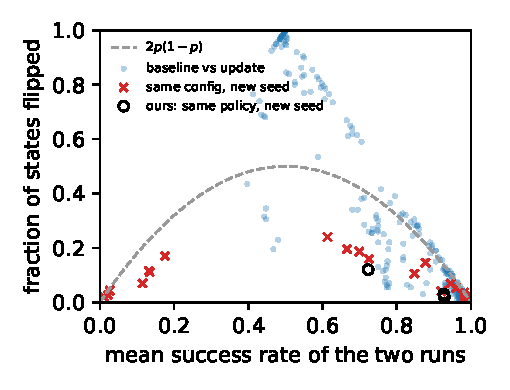
\includegraphics[width=0.55\linewidth]{fig_noise_floor.pdf}
  \caption{Fraction of states that change outcome between two runs, against their mean success
  rate. Crosses: the same configuration with a new seed. Dots: baseline against every other
  configuration in VLAQuantBench. The dashed curve is $2p(1-p)$, the flip rate if every state had
  success rate $p$; repeats fall below it because states differ in difficulty.}
  \label{fig:floor}
\end{figure}

\section{Per-state regressions of X-VLA under quantization}
\label{sec:xvla}

\paragraph{Setup.} We evaluate \texttt{lerobot/xvla-libero} in LeRobot 0.6.1 on LIBERO-10:
10 tasks $\times$ 10 initial states $\times$ 5 rollouts, absolute end-effector control, 10
flow-matching steps, and LeRobot's 520-step limit. Every failure in the FP32 run is a timeout at
this limit; VLAQuantBench allows 900 steps and reports 97.9\% for the same model, against 92.4\%
here. The quantized variants round all 267 linear layers (792M parameters) to a symmetric
integer grid and store them dequantized: INT8 with one scale per output channel, INT4 with one
scale per group of 128 inputs.

\begin{table}[t]
  \centering
  \small
  \caption{X-VLA on LIBERO-10, FP32 against each variant: 100 states, 5 rollouts each. Naive
  flips use the first rollout only (to failure / to success). BH: states with a significant
  per-state change at FDR 0.1 (regressed / improved). The first two rows compare FP32 with
  itself.}
  \label{tab:xvla}
  \begin{tabular}{lccccc}
    \toprule
    Variant & Success & $\Delta$ [95\% CI] & Naive flips & BH & $P(\text{worse})>0.9$ \\
    \midrule
    FP32, new policy seeds & .928 & $+0.2$ [$-1.0$, $+1.4$] & 0 / 3 & 0 / 0 & 0 \\
    FP32, new scene seeds & .930 & $+0.4$ [$-0.4$, $+1.2$] & 0 / 2 & 0 / 0 & 0 \\
    W4, group 128 & .918 & $-0.8$ [$-3.2$, $+1.2$] & 4 / 2 & 0 / 0 & 1 \\
    W3, group 128 & .726 & $-20.0$ [$-26.8$, $-13.4$] & 23 / 2 & 7 / 0 & 26 \\
    \todo{2 denoising steps} & & & & & \\
    \todo{BF16} & & & & & \\
    \bottomrule
  \end{tabular}
\end{table}

\paragraph{The floor is low at fixed states.} With states that fix the scene seed, FP32 against
itself changes the outcome of 13 of 500 rollouts under new policy seeds and 8 of 500 under new
scene seeds; no state's success count moves by more than two, and neither run has a significant
state. 88 of the 100 states succeed in all five FP32 rollouts and 5 fail in all five. The large
seed-to-seed flip counts of Section~\ref{sec:floor} are therefore not intrinsic to the policy:
once a state is defined precisely, a rerun is close to a replay.

\paragraph{W4 is safe per state as well as on average.} Its six naive flips are twice the floor,
but none survives the test; the most affected state drops from 5/5 to 1/5 ($p=0.024$, not
significant after correction).

\paragraph{W3 fails in specific places.} The 20-point drop is concentrated: tasks 5, 8 and 9 keep
96--100\% while tasks 0, 4 and 7 lose 40--52 points. Seven states go from 5/5 to 0/5 and are
flagged; 26 have posterior probability above 0.9 of having become worse. The single-rollout
protocol would report 23 new failures and 2 new successes, and cannot say which of them are real.

\section{Discussion}

A per-state claim about a policy update is a claim about $\sim$100--200 small binomial
experiments, and it should be reported the way such claims are: with repeated rollouts, a test,
multiplicity control, and the result of the old policy against itself. We recommend reporting
per-state regressions next to $\Delta$ success whenever an update is shipped, and the noise
floor next to any per-state flip count.

\paragraph{Limitations.} Simulation only; LIBERO offers few initial states per task; our
quantization is simulated weight-only rounding. Fixed designs with $n=5$ detect only large
per-state drops: a state at 95\% success that falls to 20\% is flagged with probability 0.64 by
a single-state test at level 0.05, one that falls to 50\% with probability 0.15 (0.94 with
$n=20$). Allocating rollouts sequentially to uncertain
states~\citep{snyder2025step} is the natural next step. Related paired tests on suite
level~\citep{islam2026onnx} and update-admission gates~\citep{ma2026admission} address the
aggregate or a synthetic setting; we target states of a real VLA benchmark.

\bibliography{references}

\end{document}
"
% (see Makefile)
\documentclass{article}
\usepackage{xcolor}

\ifdefined\PREPRINT
  \usepackage[preprint]{corl_2026}
\else
  \usepackage{corl_2026}
  % The style's footer names the main conference; this is a workshop submission.
  \makeatletter
  \renewcommand{\@noticestring}{Submitted to the CoRL 2026 Workshop on Efficient Foundation
    Models for Real-Time Embodied AI. Do not distribute.}
  \makeatother
\fi

\usepackage{booktabs}
\usepackage{graphicx}
\graphicspath{{../}}
\usepackage{amsmath}
\usepackage{xspace}

\newcommand{\todo}[1]{\textcolor{red}{[TODO: #1]}}
\newcommand{\pizero}{$\pi_0$\xspace}
\newcommand{\pizerofive}{$\pi_{0.5}$\xspace}

\title{Higher Success, New Failures:\\Measuring Per-State Regressions in VLA Policy Updates}

\author{
  Qiang Guo\\
  Independent Researcher\\
  \texttt{glay.guo@foxmail.com}
}

\begin{document}
\maketitle

\begin{abstract}
Quantized, distilled or otherwise accelerated vision-language-action (VLA) policies are judged by
the change in their aggregate success rate. A deployment also needs to know whether the new policy
fails where the old one succeeded. Comparing the two policies with one rollout per initial state,
the usual protocol, cannot tell: in VLAQuantBench's public LIBERO records, rerunning an unchanged
configuration with a new seed changes the outcome of up to a quarter of the initial states. We
define a state as a LIBERO initial state together with its scene seed, roll out every state several
times per policy with common random numbers, and test each state for regression under
false-discovery control. On X-VLA in LIBERO-10, this old-versus-old floor falls to 2--3 flips per
100 states; 4-bit weights leave every state intact, while 3-bit weights break seven states
outright and concentrate a 20-point drop on a few tasks. \todo{update with the step and BF16
variants.}
\end{abstract}

\keywords{Vision-language-action models, quantization, evaluation, regression testing}

%===============================================================================

\section{Introduction}

Deployed VLA policies are updated often: weights are quantized, flow-matching policies are run
with fewer denoising steps, longer action chunks are executed open-loop, and checkpoints are
fine-tuned again. Each update is reported as a change in success rate over a benchmark
suite~\citep{xu2026vlaquantbench}. An operator who has validated the old policy on a set of
situations asks a different question: in which of them does the new policy now fail? The
question is familiar from backward compatibility of model updates in classification
\citep{bansal2019updates,srivastava2020compat,yan2021pcr}, where a more accurate model can still
err on inputs the old one got right. For closed-loop control it has not been measured with any
statistical care.

Recent work compares VLA policies initial state by initial state on
LIBERO~\citep{liu2023libero}: \citet{sawada2026paired} pair states across perturbations and find
that up to 34.5\% of them change outcome, and \citet{yardimci2026collapse} report per-task
collapse under online RL fine-tuning while the aggregate looks healthy. These comparisons use one
rollout per state. A VLA rollout is random, through the policy's sampling and the simulator's
scene randomization, so part of any per-state difference is noise. How large that part is has not
been reported.

We make three contributions.
\begin{itemize}
  \item \textbf{The noise floor of single-rollout comparisons.} From VLAQuantBench's public
    records of four VLAs on four LIBERO suites, rerunning an unchanged configuration with a new
    seed flips the outcome of 1--25\% of states, depending on the success rate
    (Section~\ref{sec:floor}). Many reported per-state changes are within this floor.
  \item \textbf{A protocol} that makes per-state comparisons testable: states that fix the scene
    seed, repeated rollouts with common random numbers, per-state exact tests with
    Benjamini-Hochberg control, and an explicit old-versus-old baseline
    (Section~\ref{sec:method}). The harness is built on LeRobot~\citep{cadene2024lerobot}.
  \item \textbf{Per-state regressions of X-VLA}~\citep{zheng2025xvla} under weight
    quantization on LIBERO-10 (Section~\ref{sec:xvla}): at precisely defined states a rerun is
    close to a replay, W4 changes no state significantly, and W3's losses sit in seven states
    that go from always to never succeeding.
\end{itemize}

\section{Method}
\label{sec:method}

\paragraph{States.} LIBERO ships a fixed file of initial states per task that sets the robot and
the movable objects. Fixtures such as cabinets and stoves, however, are placed at random each time
the scene is rebuilt: three hard resets of LIBERO-10 task 0, state 0 gave three cabinet positions.
We therefore define a state $s$ as (task, initial state, scene seed) and reset each state with
its own fixed seed.

\paragraph{Rollouts.} Each state is rolled out $n$ times per policy variant. The policy's noise
seeds are a function of the evaluation plan only (task, batch, base seed), never of the variant,
so two variants see the same random numbers (common random numbers), and a rerun of the same
plan reproduces every episode exactly.

\paragraph{Tests.} Let $k_s^{\text{old}}, k_s^{\text{new}}$ be the successes out of $n$. For each
state we compute the one-sided Fisher exact $p$-value for ``the new variant succeeds less often''
and apply the Benjamini-Hochberg procedure~\citep{benjamini1995fdr} at FDR $q=0.1$ across states.
We also report the posterior probability that $p_s^{\text{new}} < p_s^{\text{old}}$ under
uniform Beta priors, and the aggregate change with a bootstrap over states. The \emph{naive}
count uses repeat 0 only: states that succeed under the old variant and fail under the new one, as
a single-rollout protocol would report.

\paragraph{Noise floor.} The old policy is compared with itself: the same states and scene seeds,
new policy seeds. Any flip or regression found here is a false alarm by construction.

\section{How noisy is one rollout per state?}
\label{sec:floor}

VLAQuantBench~\citep{xu2026vlaquantbench} released every episode of its 409 closed-loop runs
(MIT licence). On LIBERO it runs each configuration once on 200 states (20 initial states for
each of 10 tasks; 190 for X-VLA), and 20 configurations again with seeds 1 and 2. We use commit
\texttt{4a2cb7c}.

\paragraph{Unchanged configurations flip many states.} Table~\ref{tab:floor} and
Figure~\ref{fig:floor} show the states whose outcome differs between two seeds of the same
configuration. Near the ceiling the count is small (1--8 of 200 at 97.5--99.5\% success), but it
grows quickly as success falls: 21--32 states at 72--88\%, and 32--50 at 60--71\%.

\paragraph{Seeds do not pair configurations.} Two different configurations run with the same seed
disagree on as many states as with different seeds (e.g.\ \pizerofive base against its W4A4
action-head variant on LIBERO-Object: 77.3 at the same seed, 78.0 across seeds), so seed-to-seed
flips are the right floor for VLAQuantBench's cross-configuration comparisons.

\paragraph{States do differ.} The flips are not only noise around a common rate. For \pizerofive
with a W4A4 action head on LIBERO-Object (61\% success), 43 states fail in all three seeds and 85
succeed in all three; if all states had the same success rate we would expect 12 and 46. Real
per-state effects exist; a single rollout cannot separate them from chance.

\paragraph{Consequence.} Take \pizero~\citep{black2024pi0} on LIBERO-10 with W8 weights: aggregate
success moves from 48.5\% to 47.5\%, while 24 states flip to failure and 22 to success. At that
success rate, a new seed alone flips a comparable number of states (Table~\ref{tab:floor}). A
per-state reading of such a comparison needs repeated rollouts.

\begin{table}[t]
  \centering
  \small
  \caption{States that change outcome between seeds of the same configuration (VLAQuantBench,
  LIBERO, 200 states). Rows span the range of success rates; all 20 repeated configurations are
  in the supplementary material.}
  \label{tab:floor}
  \setlength{\tabcolsep}{4pt}
  \begin{tabular}{llccc}
    \toprule
    Suite / model & Configuration & Success by seed & Flips per seed pair & Never / always / mixed \\
    \midrule
    Object / \pizerofive & baseline & .990 .985 .995 & 5, 1, 4 & 0 / 195 / 5 \\
    Object / \pizerofive & W4A4, action head & .600 .630 .610 & 44, 50, 50 & 43 / 85 / 72 \\
    Spatial / \pizerofive & W4A4, action head & .705 .705 .685 & 44, 36, 32 & 34 / 110 / 56 \\
    Spatial / \pizerofive & W4A4, MLP only & .880 .875 & 29 & 10 / 161 / 29 \\
    10 / OpenVLA-OFT & W3, no fc2 in head & .935 .915 .910 & 8, 7, 9 & 11 / 177 / 12 \\
    \bottomrule
  \end{tabular}
\end{table}

\begin{figure}[t]
  \centering
  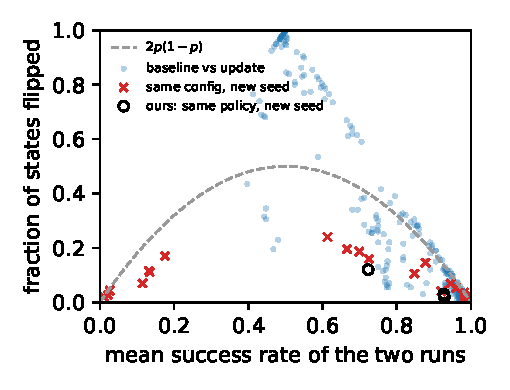
\includegraphics[width=0.55\linewidth]{fig_noise_floor.pdf}
  \caption{Fraction of states that change outcome between two runs, against their mean success
  rate. Crosses: the same configuration with a new seed. Dots: baseline against every other
  configuration in VLAQuantBench. The dashed curve is $2p(1-p)$, the flip rate if every state had
  success rate $p$; repeats fall below it because states differ in difficulty.}
  \label{fig:floor}
\end{figure}

\section{Per-state regressions of X-VLA under quantization}
\label{sec:xvla}

\paragraph{Setup.} We evaluate \texttt{lerobot/xvla-libero} in LeRobot 0.6.1 on LIBERO-10:
10 tasks $\times$ 10 initial states $\times$ 5 rollouts, absolute end-effector control, 10
flow-matching steps, and LeRobot's 520-step limit. Every failure in the FP32 run is a timeout at
this limit; VLAQuantBench allows 900 steps and reports 97.9\% for the same model, against 92.4\%
here. The quantized variants round all 267 linear layers (792M parameters) to a symmetric
integer grid and store them dequantized: INT8 with one scale per output channel, INT4 with one
scale per group of 128 inputs.

\begin{table}[t]
  \centering
  \small
  \caption{X-VLA on LIBERO-10, FP32 against each variant: 100 states, 5 rollouts each. Naive
  flips use the first rollout only (to failure / to success). BH: states with a significant
  per-state change at FDR 0.1 (regressed / improved). The first two rows compare FP32 with
  itself.}
  \label{tab:xvla}
  \begin{tabular}{lccccc}
    \toprule
    Variant & Success & $\Delta$ [95\% CI] & Naive flips & BH & $P(\text{worse})>0.9$ \\
    \midrule
    FP32, new policy seeds & .928 & $+0.2$ [$-1.0$, $+1.4$] & 0 / 3 & 0 / 0 & 0 \\
    FP32, new scene seeds & .930 & $+0.4$ [$-0.4$, $+1.2$] & 0 / 2 & 0 / 0 & 0 \\
    W4, group 128 & .918 & $-0.8$ [$-3.2$, $+1.2$] & 4 / 2 & 0 / 0 & 1 \\
    W3, group 128 & .726 & $-20.0$ [$-26.8$, $-13.4$] & 23 / 2 & 7 / 0 & 26 \\
    \todo{2 denoising steps} & & & & & \\
    \todo{BF16} & & & & & \\
    \bottomrule
  \end{tabular}
\end{table}

\paragraph{The floor is low at fixed states.} With states that fix the scene seed, FP32 against
itself changes the outcome of 13 of 500 rollouts under new policy seeds and 8 of 500 under new
scene seeds; no state's success count moves by more than two, and neither run has a significant
state. 88 of the 100 states succeed in all five FP32 rollouts and 5 fail in all five. The large
seed-to-seed flip counts of Section~\ref{sec:floor} are therefore not intrinsic to the policy:
once a state is defined precisely, a rerun is close to a replay.

\paragraph{W4 is safe per state as well as on average.} Its six naive flips are twice the floor,
but none survives the test; the most affected state drops from 5/5 to 1/5 ($p=0.024$, not
significant after correction).

\paragraph{W3 fails in specific places.} The 20-point drop is concentrated: tasks 5, 8 and 9 keep
96--100\% while tasks 0, 4 and 7 lose 40--52 points. Seven states go from 5/5 to 0/5 and are
flagged; 26 have posterior probability above 0.9 of having become worse. The single-rollout
protocol would report 23 new failures and 2 new successes, and cannot say which of them are real.

\section{Discussion}

A per-state claim about a policy update is a claim about $\sim$100--200 small binomial
experiments, and it should be reported the way such claims are: with repeated rollouts, a test,
multiplicity control, and the result of the old policy against itself. We recommend reporting
per-state regressions next to $\Delta$ success whenever an update is shipped, and the noise
floor next to any per-state flip count.

\paragraph{Limitations.} Simulation only; LIBERO offers few initial states per task; our
quantization is simulated weight-only rounding. Fixed designs with $n=5$ detect only large
per-state drops: a state at 95\% success that falls to 20\% is flagged with probability 0.64 by
a single-state test at level 0.05, one that falls to 50\% with probability 0.15 (0.94 with
$n=20$). Allocating rollouts sequentially to uncertain
states~\citep{snyder2025step} is the natural next step. Related paired tests on suite
level~\citep{islam2026onnx} and update-admission gates~\citep{ma2026admission} address the
aggregate or a synthetic setting; we target states of a real VLA benchmark.

\bibliography{references}

\end{document}
